%%%%%%%%%%%%%%%%%%%%%%%%%%%%%%%%%%%%%%%%%%%%%%%
% BEGIN BEWEGING in 3-D
%%%%%%%%%%%%%%%%%%%%%%%%%%%%%%%%%%%%%%%%%%%%%%%
\chapter{Beweging in 3-D}

In dit hoofdstuk komt beweging van objecten in 3-D aan bod. We beginnen met een kleine 
inleiding over vectoren. Zoals we zullen zien, bieden vectoren namelijk een krachtige methode om positie, snelheid en versnelling - en nog vele andere grootheden - te beschrijven. We eindigen met de beschrijving van de baan van een object in het geval van eenparig versnelde beweging.

\noindent Stof uit Giancoli:
\begin{itemize}
\item Hoofdstuk 2.1 - 2.8: beweging in 1-D
\item Hoofdstuk 3: vectoren en beweging in 3-D
\end{itemize}

\noindent Stof uit Adams:
\begin{itemize}
\item Hoofdstuk 10.2: Vectors
\end{itemize}

\section{Vectoren en scalairen}

Binnen de klassieke mechanica krijgen we te maken met twee typen variabelen {\it scalairen} en
{\it vectoren}. Een scalar is een grootheid met alleen een waarde, die niet afhangt van het co\"{o}rdinaten systeem: rotaties en translaties veranderen een scalar niet. Denk bij een scalar 
aan grootheden zoals massa of elektrische lading van een deeltje of bijvoorbeeld temperatuur. 
Voor scalaire grootheden maakt het niet uit vanuit welk standpunt je ze bekijkt ze blijven
altijd hetzelfde.

Een vector daarentegen is een grootheid die wel afhangt van wat je precies met je co\"{o}rdinatensysteem doet: naast een grootte heeft een vector een richting. De vectoren waarmee we te maken krijgen tijdens het college klassieke mechanica hebben allemaal  3-componenten: een voor de $x$, een voor de $y$ en een voor de $z$ richting. Eigenlijk elke grootheid die een betekenis heeft als 3 dimensionaal object wordt weergegeven door een vector.  Denk hierbij
bijvoorbeeld aan positie snelheid en kracht: naast een grootte is de richting van een vector 
grootheid even belangrijk. Het heeft weinig zin om het te hebben over een kracht van 10~N als
je niet erbij vertelt in welke richting, net zo min als het zin heeft een argeloze wandelaar
te vertellen dat ie nog 10~km moet lopen als je er niet bij vertelt welke kant op.

\subsection{Onze vector notatie}

Vector grootheden worden op verschillende manieren weergegeven in de tekstboeken of
andere literatuur. Vaak wordt ervoor gekozen om een vector vetgedrukt weer te geven. Dus
voor een vector $A$ krijg je dan:
\begin{equation}
{\bf A} = (A_x, A_y, A_z)
\end{equation}
Helaas is het erg lastig voor de docent en de student om 'vetgedrukt' te gaan schrijven als er een vector in het spel is, en dus komen vetgedrukte vectoren slechts voor in tekstboeken.
Een andere mogelijkheid die vaak wordt gebruikt is door een pijltje boven een vector te zetten.
Dezelfde vector $A$ wordt dan dus:
\begin{equation}
\vec{A}=(A_x, A_y, A_z)
\end{equation}
Deze laatste notatie wordt verder in het college gebruikt. Als er een oplossing van een
opgaven wordt gezocht in de vorm van een vector, wordt van jullie - de studenten - gevraagd
de vectoren ook als zodanig weer te geven.  De 'middelbare-school' varianten waarbij bijvoorbeeld snelheden posities en krachten in 1-dimensie werden genoteerd zijn vanaf nu uit den boze.

\subsection{Rekenen met vectoren}\label{sec:vectorcalculus}

Als je eenmaal weet hoe een vector er uit ziet, wil je natuurlijk ook met vectoren kunnen
rekenen. In deze paragraaf wordt - extreem kort - beschreven hoe je vectoren bij elkaar
moet optellen, van elkaar moet aftrekken, hoe je het 'in-product' van twee vectoren moet
nemen en hoe je de lengte van een vector kan uitrekenen. Handigheid met al deze 
operaties is vereist voor het soepeltjes maken van opgaven horend bij klassieke mechanica
(en speciale relativiteitstheorie).

Vectoren optellen moet component-voor-component gedaan 
worden. Stel je hebt twee vectoren $\vec{A}$ en $\vec{B}$, dan geldt voor de som van deze 
vectoren, $\vec{C}$, dus:
\begin{eqnarray}
\vec{C} & = & \vec{A} + \vec{B} \\
              & = & (A_x + B_x,\, A_y + B_y, \,A_z + B_z) 
\end{eqnarray}
Grafisch is dit optellen zoals weergegeven in Fig.~\ref{fig:vecop}~a) voor te stellen door $\vec{B}$
vast te knopen aan de kop van $\vec{A}$. 
\begin{figure}[htbp]
\begin{center}
  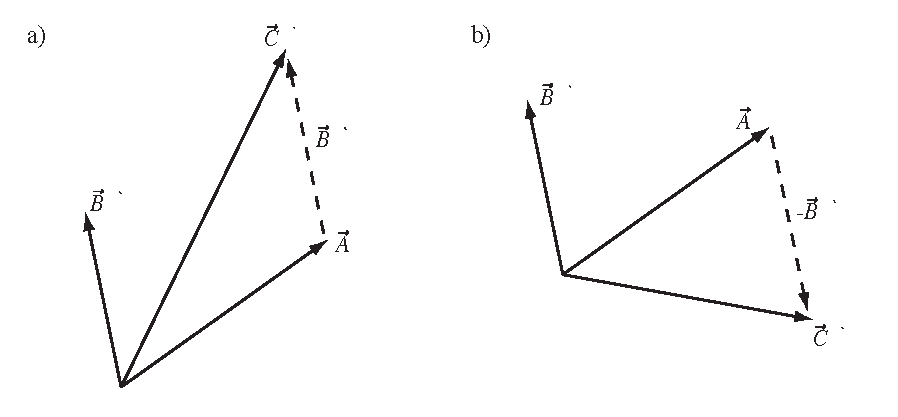
\epsfig{file=VectorOperations.pdf, width=\textwidth}
\caption{{\it (a) Optellen van vectoren. (b) Aftrekken van vectoren }}
\label{fig:vecop}
\end{center}
\end{figure}

Optellen van vectoren is bijvoorbeeld van belang
als je wil uitrekenen wat een positie van een object is na verschillende stappen te hebben
afgelegd, of voor het uitrekenen van een resultante kracht als er meerdere krachten op
ons object werken.

Voor het aftrekken van twee vectoren, $\vec{A}$ en $\vec{B}$, geldt:
\begin{eqnarray}
\vec{C} & = & \vec{A} - \vec{B} \\
              & = & (A_x - B_x,\, A_y - B_y, \,A_z - B_z) 
\end{eqnarray}
Grafisch is het aftrekken van twee vectoren weergegeven in Fig.~\ref{fig:vecop}~b). De resultante
vector $\vec{C}$ wordt verkregen door $\vec{B}$ van richting om te draaien en deze vervolgens
aan de punt van $\vec{A}$ te leggen.

De lengte van een vector kan eenvoudig worden berekend met behulp van onze klassieke
vriend Pythagoras. Voor een vector $\vec{A}$ is de lengte dus gegeven door:
\begin{equation}
|\vec{A}|  = \sqrt{A_x^2+A_y^2+A_z^2}  
\end{equation}
Met de lengte van een vector bekend, kan je vervolgens een vector maken die dezelfde
richting heeft als de originele vector $\vec{A}$, maar met lengte 1:
\begin{eqnarray}
\hat{A} & = & \frac{\vec{A}}{|\vec{A}|} \\
             & = & \left(\frac{A_x}{|\vec{A}|},\, \frac{A_y}{|\vec{A}|},\, \frac{A_z}{|\vec{A}|}\right)
\end{eqnarray}
Vectoren met lengte~1 worden {\bf eenheidsvectoren} genoemd, en ze worden onder andere
gebruikt om de richting van een vector aan te geven. Daarnaast kunnen we eenheidsvectoren gebruiken om een willekeurige andere vector te schrijven. Voor het definieren van een willekeurige vector in cartesische co\"{o}rdinaten kan het handig zijn de eenheidsvectoren te definieren, \ihat, \jhat en \khat die de richting van respectievelijk de $x$-as, de $y$-as en de $z$ aangeven.  Onze vertrouwde vector $\vec{A}$ kan met behulp van deze eenheidsvectoren worden geschreven als:
\begin{equation}
\vec{A} = (A_x,\,A_y,\,A_z) = A_x\,\ihat + A_y \, \jhat + A_z \khat
\end{equation}
Merk op dat de vectoren die we kiezen om een co\"{o}rdinatensysteem - in dit geval het cartesische - te beschrijven loodrecht op elkaar staan.  Ook bij andere keuzen van de co\"{o}rdinaten die we later in de college's tegenkomen is dit het geval. ({\it kennen jullie andere co\"{o}rdinatensystemen dan het cartesische? zo nee, zou je iets kunnen bedenken?})

Bovenstaande opmerking kunnen we formeel bewijzen door het introduceren van het vector scalar product of inproduct. Als je twee vectoren $\vec{A}$ en $\vec{B}$ hebt dan is het inproduct gedefinieerd als:
\begin{equation}
\vec{A}\cdot\vec{B} \equiv A_x B_x + A_y B_y + A_z B_z
\end{equation}
Let op de $\cdot$ tussen de twee vectoren die aangeeft dat er hier sprake is van een inproduct.
Laten we eens kijken wat het inproduct precies betekent. Ten eerste kan je opmerken dat we hier te maken hebben met een scalar. Het maakt dus niet uit hoe we tegen de vectoren $\vec{A}$ en $\vec{B}$ aankijken: we zouden bijvoorbeeld het gehele coordinatensysteem over een willekeurige hoek kunnen
draaien, waarbij $\vec{A}\rightarrow\vec{A}^{'}$ en $\vec{B}\rightarrow\vec{B}^{'}$. Wat we bedoelen met de uitspraak dat het inproduct {\it invariant} is onder een willekeurige rotatie is wiskundig niets anders dan:
\begin{equation}
\vec{A}\cdot\vec{B} = \vec{A}^{'}\cdot\vec{B}^{'}
\end{equation}
Hier kunnen we handig gebruik van maken om een diepere betekenis toe te kennen aan ons inproduct. We kunnen er namelijk voor kiezen om het coordinatensysteem zodanig te draaien dat de vector $\vec{A}^{'}$ langs de $x$-as ligt van ons nieuwe coordinatensysteem. En vervolgens kunnen we nog een keer draaien om de $x$-as totdat de vector $\vec{B}^{'}$ in het $x-y$ vlak ligt, zoals aangegeven in Fig.~\ref{fig:inproduct}.
\begin{figure}[htbp]
\begin{center}
  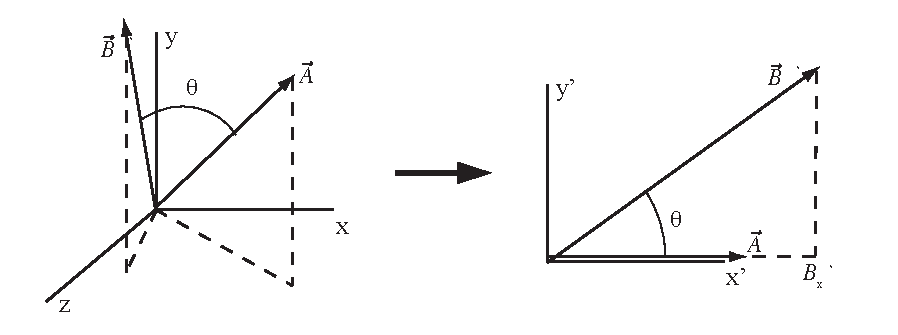
\epsfig{file=InnerProduct.pdf, width=\textwidth}
\caption{{\it Het inproduct van twee vectoren is invariant onder rotaties van het coordinatensysteem. }}
\label{fig:inproduct}
\end{center}
\end{figure} 
Voor het inproduct tussen de oude vectoren (!) geldt nu dus:
\begin{eqnarray}
\vec{A}\cdot\vec{B} & = & A_x^{'} B_x^{'} + 0 B_y^{'} + 0 B_z^{'} \\
                                   & = & |\vec{A}^{'}| |\vec{B}^{'}| \cos\theta^{'} \\
                                   & = & |\vec{A}||\vec{B}|\cos\theta \label{eq:inpr}
\end{eqnarray}
Hierbij is $\theta$ de hoek tussen de vectoren $\vec{A}$ en $\vec{B}$ en die is hetzelfde voor de geroteerde vectoren. Verder maken we er  gebruik van dat de lengte van een vector niet verandert bij een rotatie, en dat $A_x^{'}=|\vec{A}^{'}|$, omdat  deze vector langs de $x$-as wijst. Het inproduct van twee vectoren geeft je dus een manier om de hoek tussen de vectoren uit te rekenen. Daarnaast meet een inproduct de lengte van een vector in de richting van die andere vector (cryptische uitspraak die de moeite waard is om te begrijpen). 

Laten we ook eens kijken naar het inproduct van een vector met zichzelf. Aan de ene kant hebben we:
\begin{equation}
\vec{A}\cdot\vec{A} = A_x^2 + A_y^2 +A_z^2 
\end{equation}
En aan de andere kant hebben we dankzij Vgl.~\ref{eq:inpr}:
\begin{equation}
\vec{A}\cdot\vec{A} = |\vec{A}||\vec{A}|\cos 0 = |\vec{A}|^2
\end{equation}
En dat is gelukkig hetzelfde. Het inproduct van een vector met zichzelf geeft je dus de lengte van die vector in het kwadraat.
                                    
Tenslotte kan je direct aan het inproduct zien dat de eenheidsvectoren, \ihat, \jhat en \khat loodrecht op elkaar staan omdat:
\begin{equation}
\ihat\cdot\jhat=\ihat\cdot\khat=\jhat\cdot\khat = 0
\end{equation}
En dus klopt de belofte die we hierboven hebben gemaakt.

\section{Positie}

De eerste natuurkundige vector die we tegenkomen geeft de coordinaat van een object aan. We zullen voor een positie van een object in het kader van dit college altijd (of in ieder geval zoveel mogelijk) de volgende notatie aanhouden:
\begin{equation}
\vec{r}  \equiv (x, y, z)
\end{equation}
Niet echt wonderlijk, maar we kiezen ervoor om $x$, $y$ en $z$ te gebruiken voor de coordinaten.
Uiteraard kunnen we de positie ook weer schrijven als een som van eenheidsvectoren. Ten overvloede:
\begin{equation}
\vec{r} = x \ihat + y \jhat + z \khat
\end{equation}
Vaak zijn we niet direct geintereseerd in een positie zelf, maar in een verandering in positie. Een vector die je vaak tegenkomt in dat kader is de verplaatsingsvector, \dr, die is gedefinieerd als:
\begin{equation}
\dr \equiv \vec{r}_2 - \vec{r}_1
\end{equation}
De verplaatsingsvector wordt simpelweg verkregen door het aftrekken van twee vectoren zoals beschreven in de vorige paragraaf. Zoals duidelijk is in Fig.~\ref{fig:vecop}~b) wijst de vector \dr in de
richting van de $\vec{r}_2$ gezien vanaf de punt van $\vec{r}_1$. De vector \dr krijgt een duidelijke betekenis als we dadelijk posities definieren die veranderen als functie van de tijd ({\it wat zouden 
zulke vectoren ook alweer voorstellen?}).

\section{Snelheid en Impuls}

Een verandering van positie per eenheid van tijd kennen we uiteraard als snelheid. Om precies te zijn de instantane snelheid is gedefinieerd als de afgeleide van de positie naar de tijd. Dus de snelheid is:
\begin{equation}
\vec{v} \equiv \frac{d\vec{r}}{dt} = \left(\frac{dx}{dt}, \frac{dy}{dt}, \frac{dz}{dt}\right)
\end{equation}
Let er op dat snelheid net als de positie een vector grootheid is. Als je bij bijvoorbeeld een auto spreekt over de maximum snelheid die het beestje kan bereiken dan praat je over de maximale grootte die deze vector kan bereiken:
\begin{equation}
|\vec{v}| = \sqrt{\vec{v}\cdot\vec{v}}
\end{equation}
In het engels is het onderscheid tussen de grootte van de snelheid ('speed') en de vector snelheid ('velocity')  duidelijker. En ook als je een verschil in snelheid wil uitrekenen, moet je net
als voor de positie het verschil tussen twee snelheidsvectoren berekenen:
\begin{equation}
\dv = \vec{v}_2 - \vec{v}_1
\end{equation} 
De snelheid is uiteraard een extreem belangrijke grootheid als je een fysich systeem wil beschrijven. Vaker nog dan de snelheid zelf gebruiken natuurkundigen het begrip impuls. In de klassieke mechanica is de impuls niets anders dan de snelheid van een object  maal zijn massa:
\begin{equation}
\vec{p} \equiv m \vec{v}
\end{equation}
De impuls is als het ware een maat voor de 'hoeveelheid beweging'. Een van de redenen dat impuls zo'n enorm belangrijke grootheid is, is dat impuls ook buiten de klassieke mechanica universeel kan worden gebruikt, terwijl snelheid soms minder bruikbaar is. Het blijkt dat impuls een zogenaamde behouden grootheid is (dat zien we later in college nog weer terug) en dat er een mooie relatie is tussen impuls en het begrip kracht dat we in het volgende hoofdstuk behandelen.

\begin{center}
\line(1,0){250}
\end{center}
\begin{voorbeeld} 
\label{ex:student}
Op weg naar zijn vakantie in Spanje besluit een student op het dak van de bus te klimmen om 
indruk te maken op zijn jaarclubgenootjes. De bus rijdt met snelheid $v_b$ en de student klimt met 
snelheid $v_h$ op het dak van de bus. Wat is zijn snelheid ten opzichte van een argeloze 
toeschouwer? En onder welke hoek beweegt ie?

{\bf Oplossing} {\it We kiezen ervoor om de bus te laten rijden in de $x$-richting, 
dus $\vec{v}_b=(v_b,\,0,\,0)$
en de student klimt met snelheid $\vec{v}_s = (0,0,v_s)$ op het dak. Een stilstaande toeschouwer 
ziet de student dus met $v = (v_b,\,0,\,v_s)$ bewegen. Voor de hoek waaronder de student 
beweegt geldt nu dus eenvoudig: $\tan\theta = v_s / v_b$. Als de toeschouwer zelf ook nog 
beweegt kan je de snelheidsvector van zijn eigen beweging er ook nog bij optellen en zo voorts
}
\end{voorbeeld}

\begin{center}
\line(1,0){250}
\end{center}

\section{Versnelling}

De laatste vector die je nodig hebt om de beweging van een deeltje te karakteriseren is de 
zogenaamde versnelling. Een versnelling is niets anders dan de verandering van snelheid per 
eenheid van tijd. Deze is dus gedefinieerd als de eerste afgeleide naar de tijd van de snelheid, en 
dus de tweede afgeleide naar de tijd van de positie:
\begin{equation}
\label{eq:a}
\vec{a} \equiv \frac{d\vec{v}}{dt} = \frac{d^2\vec{r}}{dt^2} = \left(\frac{d^2x}{dt^2}, \frac{d^2y}{dt^2}, 
\frac{d^2z}{dt^2}\right)
\end{equation}
Versnelling is een begrip dat lastiger is dan het er op het eerste gezicht uitziet: zeker als je met de 
vectoren aan de slag gaat. Je zou op het eerste gezicht denken dat een versnelling altijd gepaard 
gaat met een verandering van de grootte van de snelheid, maar dit is niet altijd het geval. Dit is 
alvast een voorwaarschuwing dat je goed moet uitkijken met versnellingen en het is aan jullie om 
eens te denken onder welke omstandigheden een versnelling de grootte van de snelheid 
onveranderd laat. In ieder geval is het zo dat als de versnelling gelijk is aan nul een object beweegt 
met een {\it constante} snelheid in een {\it rechte} lijn.


\section{Eenparig versnelde beweging} \label{sec:eenparig}

Onder een eenparig versnelde beweging verstaan we een beweging waarvoor de
versnelling $\vec{a}$ constant is. Als $\vec{a}$ bekend is dan kunnen zowel de snelheid
$\vec{v}$ als de positie $\vec{r}$ worden uitgerekend als functie van de tijd, $t$. 

Laten we eerste eens kijken naar de snelheid als functie van de tijd. Stel dat op tijdstip
$t=t_0$ de snelheid $\vec{v}=\vec{v}_0$ bekend is, dan kunnen we door te integreren de 
snelheid uitrekenen als functie van de tijd ({\it let op de variabelen: er komen zowel $t$ als $t'$
voor in de vergelijkingen! weet je waarom?}) :
\begin{eqnarray}
\vec{v}(t) - \vec{v}_0 & = & \int_{t^{'}=t_0}^{t^{'}=t} \vec{a} \, dt^{'} \Rightarrow \\
\vec{v}(t)                     & =  & \vec{a} \, (t-t_0) + \vec{v}_0
\end{eqnarray}
Dus als je op $t=t_0$ de snelheid van een object weet, en je weet dat de versnelling constant is,
dan kan je de snelheid op een willekeurig tijdstip oplossen! De plaats als functie van de tijd 
kan worden bepaald door de snelheid nogmaals te integreren:
\begin{eqnarray}
\vec{r}(t) - \vec{r}_0 & = & \int_{t^{'}=t_0}^{t^{'}=t} \vec{v}\,dt^{'} \\
                                   & = &  \int_{t^{'}=t_0}^{t^{'}=t}  (\vec{a} \, (t^{'}-t_0) + \vec{v}_0) \,dt^{'} \Rightarrow \\
\vec{r}(t)                    & = & \frac{1}{2} \vec{a} (t-t_0)^2 +\vec{v}_0 \,(t-t_0) + \vec{r}_0 \label{eq:rt}
\end{eqnarray}
Deze vergelijking beschrijft eenparig versnelde beweging gegeven een beginsnelheid en positie. 
Waarschijnlijk heeft een aanzienlijk deel van jullie deze vergelijking al gezien op de middelbare school 
voor beweging in 1-D en met $t_0=0$.  In vectorvorm is de vergelijking algemeen geldig in 3-D.
Uiteraard wordt de situatie een stuk ingewikkelder als de versnelling niet constant
is. De integralen kunnen dan niet meer zo mooi worden opgelost: het is de moeite je te realiseren
dat eenparig versnelde beweging eerder een uitzondering is dan regel. De reden dat eenparig
versnelde beweging toch veel aandacht krijgt is dat de oplossing eenvoudig is: een simpele parabolische baan.

Voor alle duidelijkheid: wat we hierboven hebben gedaan is het oplossen van een $2^{\mathrm{e}}$ orde 
differentiaalvergelijking, namelijk  Vgl.~\ref{eq:a} . Een vergelijking dus waarin dubbele afgeleiden naar de tijd 
van de positie voorkomen. Een van de dingen die je ziet is dat je voor een complete oplossing van $\vec{r}(t)$ dan ook 2 
randvoorwaarden nodig hebt. In ons geval zijn dat $\vec{v}_0$ en $\vec{r}_0$. Een standaard methode om na te gaan of de
gevonden oplossing juist is, is (i) het expliciet invullen van de randvoorwaarden en (ii) het invullen van de oplossing in de
oorspronkelijke differentiaalvergelijking. 

\begin{center}
\line(1,0){250}
\end{center}

\begin{voorbeeld} 
\label{ex:parabool}
Een kogel wordt op $t=t_0$ afgeschoten vanaf positie $\vec{r}_0 = (x_0,\,y_0,\,0)$ met beginsnelheid 
$|\vec{v}_0=v_0$ onder een hoek $\theta$ zoals aangegeven in Fig.~\ref{fig:ex1}. Bereken (i) $\vec{r}(t)$, (ii) de 
tijd $T$ waarop de kogel de grond ($z=0$) weer raakt, en (iii) de snelheid waarmee de kogel de grond raakt. 
\begin{figure}[htbp]
\begin{center}
  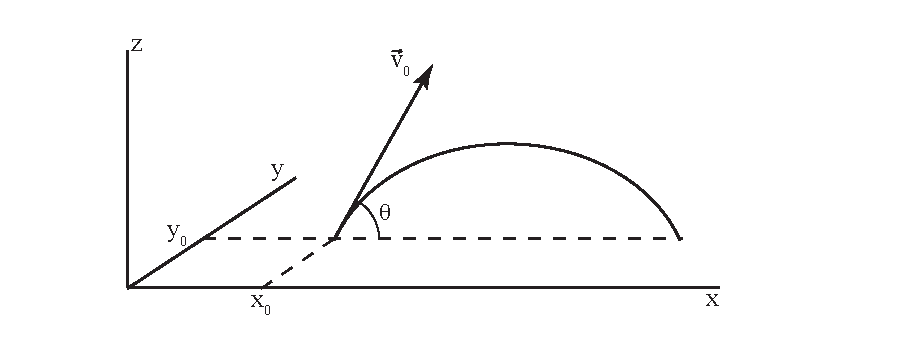
\epsfig{file=Paraboolbaan.pdf, width=\textwidth}
\caption{{\it Kogelbaan. }}
\label{fig:ex1}
\end{center}
\end{figure} 

{\bf Oplossing} {\it (i) Neem aan dat alleen de zwaartekrachtsversnelling $\vec{a}=(0,\,0,\,-g)$ een rol speelt in 
deze beweging. De snelheid $\vec{v}_0$ kan worden berekend uit de hoek $\theta$ en $v_0$ als 
$\vec{v_0} = v_0 (\cost,\,0,\,\sint)$. Invullen in vgl.~\ref{eq:rt} levert ons voor de 3 componenten 
van de positie:
\begin{equation}
\vec{r}(t) =
\left(\begin{array}{c}
0 \\
0 \\
-\frac{1}{2}\, g\,\dt^2
\end{array}\right)
+
\left(\begin{array}{c}
v_0 \cost \, \dt\\
0 \\
v_0 \sint \, \dt
\end{array}\right) 
+
\left(\begin{array}{c}
           x_0 \\
           y_0 \\
           0     \\
\end{array}\right)
\end{equation}
Met $\dt = t-t_0$. Je ziet dat we door het gebruik van vectoren te maken hebben met drie vergelijkingen (i.p.v. maar 1)
en dat ze alledrie verschillend zijn. De waarde van $y$ is constant: er is geen initiele snelheid in de $y$ richting en ook 
geen versnelling. De $x$ waarde neemt lineair toe met de tijd, omdat er een initiele snelheid is in de $x$ richting, maar
geen versnelling. Alleen de $z$ coordinaat wordt beschreven door een parabool, omdat de versnelling alleen in de $z$
richting wijst. (ii) Nu berekenen we de tijd waarop de kogel weer de grond raakt. Als de kogel de grond raakt geldt $z=0$,
ofwel:
\begin{eqnarray}
0 & = & -\frac{1}{2} g \dt^2 + v_0 \sint \dt \Rightarrow \\
\dt = 0 & \vee & \dt = \frac{2 v_0 \sint}{g}
\end{eqnarray}
De eerste oplossing komt overeen met het moment van afschieten van de kogel. De $z$ positie is 
dan immers  nul (randvoorwaarde). De tweede oplossing komt overeen met het moment dat de 
kogel de grond weer raakt (vraag: kloppen
de eenheden?). (iii) Doe dit zelf maar eens.
}
\end{voorbeeld}

\begin{center}
\line(1,0){250}
\end{center}

\section{Wat moet ik weten en kunnen?}

De volgende begrippen moet je tot je nemen:
\begin{itemize}
\item Verschil tussen vectoren en scalairen.
\item Wat zijn eenheidsvectoren?
\item Wat is de relatie tussen $\vec{r}$, $\vec{v}$ en $\vec{a}$?
\item Eenparig versnelde beweging.
\end{itemize}
En hiermee moet je kunnen rekenen:
\begin{itemize}
\item Vectoren: optellen, aftrekken en inproduct.
\item Banen van eenparig versnelde objecten.
\end{itemize}

\section{Opdrachten}

Hint voor het maken van de opgaven uit Giancoli: vervang alle getallen door variabelen. Op het 
tentamen wordt van je verwacht dat je kan rekenen met symbolen. Specifiek voor de vragen over 
objecten in een paraboolbaan: neem aan dat de zwaartekracht-versnelling wordt gegeven door $
\vec{a} = -g~\khat$.
\begin{enumerate}
\item Je kan alle opgaven bij Hfd.3 van Giancoli proberen te maken.
\item Speciale selectie uit Hfd.3 "General Problems". In ieder geval maken: 72, 75, 77, 78, 81, 83~(moeilijk),  87, 88, 93, 95.   
\item Bewijs vgl.~\ref{eq:inpr}.
\item Bewijs dat vgl.~\ref{eq:rt} zowel voldoet aan de differentiaalvergelijking in vgl.~\ref{eq:a} als 
aan de randvoorwaarden.
\item Onder welke hoek $\theta$ komt de kogel in voorbeeld~\ref{ex:parabool} het verste in $x$? 
(Hint: gebruik $\sin 2\theta = 2\sin\theta\cos\theta$.)
\item Geef een uitdrukking voor de afgelegde afstand $\Delta x$ in voorbeeld~\ref{ex:parabool} 
wanneer de kogel niet vanaf $z=0$, maar vanaf hoogte $h$ wordt afgeschoten.
\item Bereken weer de hoek $\theta$ waaronder de kogel het verste komt.
\end{enumerate}

%%%%%%%%%%%%%%%%%%%%%%%%%%%%%%%%%%%%%%%%%%%%%%%
% EINDE BEWEGING in 3-D
%%%%%%%%%%%%%%%%%%%%%%%%%%%%%%%%%%%%%%%%%%%%%%%
